\documentclass[11pt,a4paper]{report}
\usepackage[utf8x]{inputenc}
\usepackage[T1]{fontenc}
\usepackage{lmodern}
\usepackage{ucs}
\usepackage{amsmath}
\usepackage{amsfonts}
\usepackage{amssymb}
\usepackage{fullpage}
\usepackage[french]{babel}
\usepackage{xcolor}
\usepackage[pdftex]{graphicx}
\usepackage{titlesec}
\usepackage{cite}
\usepackage{pdfpages}
\usepackage{url}
\usepackage{rotating}


%%%%%%%%%%%%%%%%%encadrementdes chapitres%%%%%%%%%%%%%%%%%%%%%%%
\titleformat{\chapter} % commande de sectionnement affectée
[frame] % une des formes prédéfinies
{\itshape} % format appliqué au titre dans son ensemble
{\filright\small\enspace Chapitre \thechapter\enspace} % format du « n° » du titre
{8pt} % distance (horiz. ou vert.) entre le n° et le texte du titre
{\Large\bfseries\filcenter} % format appliqué au texte du titre
%%%%%%%%%%%%%%%%%%%%%%%%%%%%%%%%%%%%%%%%%%%%%%%%%%%%%%%%%%%%%%%%
\newcommand{\HRule}{\rule{\linewidth}{0.5mm}}
\begin{document}
%raccourcis/newcommand%

\newcommand{\cme}{cryo-MET}
\newcommand{\java}{Java~{\tiny \texttrademark}}
\newcommand{\js}{JavaScript}
\newcommand{\imj}{ImageJ}
\newcommand{\blue}{\color{red}}
\newcommand{\black}{\color{black}}

%\documentclass[10pt,a4paper]{report}
%\usepackage[utf8x]{inputenc}
%\usepackage{ucs}
%\usepackage{amsmath}
%\usepackage{amsfonts}
%\usepackage{amssymb}
%\usepackage{fullpage}
%\usepackage[french]{babel}
%\usepackage{xcolor}
%\usepackage{graphicx}
%\newcommand{\HRule}{\rule{\linewidth}{0.5mm}}
%\begin{document}

\begin{titlepage}

\begin{center}


% Upper part of the page

\includegraphics[width=0.15\textwidth]{logounibdx.png}\\[1cm]    

\textsc{\LARGE Université de Bordeaux}\\[1.5cm]
\vspace*{0.5cm}
%\textsc{\Large Projet Tutoré}\\[0.5cm]
\textsc{\Large Initiation à la Recherche\\\ et/ou Développement}\\[0.5cm]
%\textsc{\Large Development Project}\\[0.5cm]

\vspace*{1cm}

% Title
\HRule \\[0.4cm]
{ \huge \bfseries Cahier des charges}\\[0.4cm]

\HRule \\[1.5cm]
% Author and supervisor
\begin{minipage}{0.4\textwidth}
\begin{center} \large
%\emph{Author:}\\
Thomas \textsc{Faux}\\
Charlotte \textsc{Héricé}\\
Typhaine \textsc{Paysan-Lafosse}\\
Joris \textsc{Sansen}\\
\end{center}
\end{minipage}
\begin{minipage}{0.4\textwidth}
\begin{flushright} \large
%\emph{Supervisor:} \\
M. Jean-Christophe\textsc{Taveau}
\end{flushright}
\end{minipage}

\vfill

\begin{center}
2011-2012
\end{center}
% Bottom of the page

\includegraphics[width=0.4\textwidth]{./banniere_cbmn.png}\\[1cm]    
CBMN - UMR 5248 \\
B8 AVENUE DES FACULTÉS \\
F-33402 TALENCE CEDEX \\

%{\large \today}

\end{center}

\end{titlepage}
%\end{document}


\tableofcontents

\thispagestyle{empty}%%%%% empeche l'affichage du numero de page uniquement sur cette page
%\setcounter{page}{0}%%%%%% defini cette page (sommaire) comme la page 0

\chapter{Contexte}
\section{Sujet}
\paragraph*{}
Le laboratoire de Chimie et Biologie des Membranes et Nanoobjets de bordeaux (CBMN~\cite{cbmn:url}) est un laboratoire de recherche public composé de douze équipes de recherche dont l'équipe \emph{Architecture des Complexes Membranaires et processus cellulaires} (ACMPC).%
\paragraph*{}
Cette équipe, dirigée par O. Lambert s'intéresse à l'architecture de complexes membranaires sur des structures de type protéine-liposome. C'est dans ce cadre d'étude que les chercheurs travaillent avec un \emph{cryo-microscope électronique à transmission} (\cme) afin d'obtenir des micrographes des structures étudiées puis de les analyser.

\noindent
De plus, dans le cadre de leur partenariat avec une entreprise pharmaceutique, ils préparent des échantillons de virus pour observations au \cme\ et analyse. Cependant la nouvelle génération des appareils d'observations permettent une collecte de données à haut débit, avantage non négligeable mais qui pose le problème du traitement des données collectées.%

\noindent
L'automatisation du traitement des données devient alors nécessaire, l'analyse manuelle des données récupérées étant extr\^emement fastidieuse et chronophage.%

\paragraph*{}
Dans le cadre de leurs recherches et pour la partie qui nous concerne, l'analyse correspondra au traitement des images récupérées du \cme\ et plus particulièrement au \emph{picking} c'est-à-dire à le piquage des particules présentes sur les micrographes obtenus.%

\section{Objectifs}
Notre objectif consistera donc en la création donc en l'implémentation d'une méthode de picking automatisé des particules sur les micrographes. Les échantillons qui nous serviront de tests seront de deux types :%
\begin{itemize}
\item des micrographes d'échantillons de virus, de forme ronde, qu'il faut sélectionner afin de pouvoir déterminer leurs nombre et tailles,
\item des micrographes de protéines membranaires, de forme pyramidale, qu'il faudra aussi sélectionner.
\end{itemize}
\paragraph*{}
Ce procédé de piquage sera implémenté sous la forme d'un plugin ImageJ~\cite{imagej:url} qui servira de plate-forme de picking : il proposera à l'utilisateur d'utiliser des algorithmes de picking pré-installés ou d'en ajouter de nouveaux. Cela permettra de simplifier et de centraliser l'accès aux outils de sélection que l'on peut implémenter sur ImageJ.%

\paragraph*{}
Le logiciel ImageJ a été choisis car c'est un logiciel de traitement et d'analyse d'images développé en \java~\footnote{\java\ est un langage orienté-objet développé par Oracle~\cite{java:url}} par le Nation Institute of Health (NIH).%

\noindent
Ce logiciel est "open-source"~\footnote{son code source est en accès libre et est modifiable(licence GNU-GPL)}, multi-plateforme et bien connu de la communauté scientifique car initialement conçu pour des applications biomédicales. Il s'est peu à peu démocratisé dans d'autres domaines pour sa facilité d'utilisation et les possibilités de développement qu'il offre.%

\noindent
En effet, il est possible de développer soit-même et assez facilement des plugins, que ce soit en \java\ ou en \js ~\footnote{\js est un langage de programmation de script orienté objet à prototype~\cite{javascript:url}}.
\chapter{\'Etat de l'existant}
\section{Détection à l'aide de références}
\paragraph*{}
Les approches initiales concernant la piquage de particules furent basées sur des références faisant appel à un modèle. Cette technique est utilisée pour trouver de petites parties d'une image en la comparant à un modèle. Celui-ci peut \^etre obtenu soit à partir d'une structure tridimensionnelle connue si elle est utilisable soit par sélection d'une particule servant d'exemple dans le micrographe. L'algorithme détermine la meilleure correspondance entre la cible et le modèle pour pouvoir le localiser dans l'image.%ensuite la meilleure localisation du modèle en le testant dans l'image cible afin qu'il puisse correspondre le mieux possible \blue afin qu'il corresponde au maximum?\black.%

\noindent
La détéction par un modèle de référence est aujourd'hui plus performante, elle a été améliorée en tenant compte des changements d'efficacité de la variance locale dans l'espace de Fourier et de nouvelles approches qui utilisent différentes méthodes pour incorporer des modèles de bruit générique, ceci afin de pouvoir mieux gérer le bruit.%

% take a different way to incorpore generic noise model.%

\section{Piquage de particules sans références}
\subsection{Détection des bords et transformée de Hough}
%$\textcolor{red}{(ref:Automatic Particle Detection Through Efficient Hough Transforms 
%by Yuanxin Zhu, Bridget Carragher, Fabrice Mouche, and Clinton S.Potter
%IEEE TRANSACTIONS ON MEDICAL IMAGING,VOL.22,N0.9,September 2003)}$\\


%$\textcolor{red}{(ref:http://en.wikipedia.org/wiki/Hough_transform)}$\\
\paragraph*{}
Les difficultées majeures rencontrées dans les techniques basées sur la détection des contours sont dues à la compléxité de détecter les bords des particules lorsqu'il y a un bruit de fond important sur les images issues de la Microscopie à Transmission Electronique.%

\noindent
Cette technique est basée sur la détection des arêtes ainsi que sur l'application de la transformée de Hough~\cite{PdetectEHT:article}. Cette méthode permet de détecter la présence de formes comme des lignes, des cercles ou encore des ellipses.%

\noindent
Dans la transformée de Hough\cite{HT:url}, chaque ligne correspond à un vecteur à deux paramètres: $\Theta$ (angle) et $\rho$ (norme du vecteur).
Cette technique est basée sur la transformation de toutes les lignes possibles qui passent par un point, c’est-à-dire en calculant la valeur de $\rho$ pour chaque $\Theta$, on obtient alors une sinusoïde unique appelée espace de Hough. Si les courbes associées à deux points se coupent, l'endroit où elles se coupent dans l'espace de Hough correspond aux paramètres d'une droite qui relie ces deux points.%

\paragraph*{}
La détection de formes s’apparentant à des cercles ou des axes circulaires implique la localisation de tous les centres possibles et de trouver le rayon pour chaque centre ciblé.

\noindent
Si le rayon du cercle est déjà connu, les coordonnées probables du centre du cercle sont d'abord stockées dans un fichier. Elles sont ensuite recherchées dans l'image afin de déterminer les points indiquant la localisation du centre des particules circulaires.%

\noindent
Inversement, si le rayon des particules n'est pas connu, un seul paramètre en plus est nécessaire. Il suffit d'enregistrer, non pas un seul point pour chaque pixel de contour mais une ligne constituée de plusieurs points le long du contour de la particule dans ce plan.%

\paragraph*{}
D'autre part, pour détecter des particules de formes irrégulières, l'approche décrite précédemment peut également \^etre utilisée mais la transformée de Hough devra alors \^etre remplacée par la transformée de Hough Généralisée~\cite{GHT:url}. 
Cette nouvelle méthode repose sur la modification de la transformée de Hough en utilisant le principe de l'identification à partir d'un modèle de référence. Cette modification permet également d'utiliser la transformée de Hough pour la détection d'objets non caractérisés à l'aide d'une équation analytique.%
%$\textcolor{red}{(ref:http://en.wikipedia.org/wiki/Generalised_Hough_transform)}$\\

\noindent
Tout d'abord, la méthode requiert la sélection de deux paramètres: la localisation du point à l'aide d'un modèle de forme.
Ensuite, une distance adéquat est bougée dans différentes directions $\rho$ afin d'arriver au point L. Pour détecter les  particules orientées différemment ou qui ne seraient pas à la m\^eme échelle par rapport à une m\^eme forme, l'ajout de deux paramètres est nécessaire : l'orientation et l'echelle.

\subsection{DoGLFC et classement par affinité}
%$\textcolor{red}{(ref: Reference-free particle selection enhanced with semi-supervised machine learning for cryo-electron microscopy
%by Robert Langlois, Jesper Pallesen, Joachim Frank
%Journal of Structural Biology 175, (2011)353-361)}$
\paragraph*{}
Cette technique est basée sur l'utilisation de l'algorithme DoGLFC\footnote{Difference Of Gaussian Local Fast Correlation} complété par l'algorithme de classement par affinité~\cite{DoGAff:article}.

\paragraph*{}
Le DoGLFC est basé sur l'algorithme DoG Picker du Scripps Institute\cite{Scripps:url}, une méthode rapide qui permet la segmentation de particules. Après l'application de l'algorithme de Différence de Gauss (DoG), on obtient une cartographie de points similaire à celle de la méthode utilisant un modèle de référence.%\blue {\Large ?!} \black %

\noindent
Cet algorithme requiert un paramètre ajustable unique ou un jeu de paramètres basé sur le rayon de la particule ou un ordre de grandeur du rayon. L'exécution de cet algorithme renvoie une liste de trois paramètres décrivant la localisation de la particule (les coordonnées \emph{x} et \emph{y}) et la taille du pic.%

\noindent
L'algorithme DoGLFC sélectionne les particules (ou objets) potentielles de taille déterminée, ceci a un pouvoir discriminatif moindre par rapport à une technique basée sur une référence, tel que l'utilisation d'un modèle de référence, mais elle ne nécessite pas d'avoir beaucoup d'informations pour que la référence soit utilisable comme modèle.%

\paragraph*{}
Pour améliorer le rendement lors du piquage des particules, un nouvel algorithme semi-supervisé, le classement par affinité, peut \^etre appliqué.

\noindent
L’algorithme a besoin de trois paramètres d'entrée: un jeu d'images, la taille maximale de chaque vecteur et deux jeux d'indices indiquant quelle fen\^etre doit \^etre utilisée comme référence positive ou négative.

\noindent
Lorsque l'algorithme a fini de se dérouler, on obtient une note de classement de chaque fen\^etre où ce dernier est le plus proche de celui de la fen\^etre où se trouve la particule ciblée.

\paragraph*{}
L'utilisation de DoGLFC complété par le classement par affinité permet d'extraire
rapidement les particules de l'image et d'éliminer avec précision les particules correspondant à de la contamination ou du bruit de fond.

\section{Perceptron}

\paragraph*{}
Un perceptron est une sorte de réseau neuronal artificiel. Dans son état le plus simple, il représente un système de classification binaire/linéaire.%

\noindent
Ce programme a la particularité d'être capable d'apprendre des concepts, ce qui signifie qu'il peut apprendre afin de répondre par vrai ou faux à des données qui lui sont soumises, gr\^ace à la présentation répétée de plusieurs exemples d'étude.
Il a déjà été testé sur des images binaires pour la détection de formes ou de contours mais pas sur des images en niveaux de gris ou sur des problèmes de reconnaissance de modèles visant à sélectionner des particules. Le réseau neuronal n'a pas non plus été exploité comme un outils de sélection automatique de particules mais plusieurs recherches ont conclu qu'il pourrait \^etre utilisé pour l'élimination de faux-positifs.~\cite{Perceptron:article}.%


\chapter{Analyse des besoins}

\section{Besoins fonctionnels}
\subsection*{Le plugin}
\begin{itemize}
\item Au lancement, les images seront préalablement chargées sur \imj , et l'utilisateur aura le choix entre plusieurs algorithmes de picking qui lui proposeront les différents traitements applicables afin d'optimiser le piquage,
\item l'interface proposera un mode de prévisualisation afin de vérifier les changements apportés à l'image avant de les appliquer au stack,
\item l'affichage sera clair et succinct, et sera constitué d'une liste de boutons, scrollbars, et autres paramètres modifiables (rayons de filtres, etc),
\item les résultats seront affichés dans un tableau, et visualisables sur le stack afin de vérifier le bon déroulement du processus,
\item l'utilisateur pourra modifier les sélections (ajouter et retirer les pointeurs),
\item il devra également être possible d'implanter simplement de nouveaux algorithmes dans l'interface.


\end{itemize}
\subsection*{Les algorithmes}
\begin{itemize}
\item Traitements et segmentation des micrographes issus de \cme,
\item piquage automatique des particules depuis les micrographes,
\item le format de sortie est un jeu de coordonnées \emph{x,y} associé à la position de l'image dans le stack, le tout enregistré dans un fichier au format \emph{.csv}.
\end{itemize}
\section{Besoins non fonctionnels}
\subsection*{Le plugin}
\begin{itemize}
\item L'implémentation de la plateforme sera faite en \java,
\item nous utiliserons les API\footnote{Application Programming Interface} graphiques de la bibliothèque \emph{swing},
\item le programme devra être le plus simple d'utilisation possible afin de le rendre accessible à tous,%même les moins bon
\item le code devra être suffisamment clair, explicite et commenté afin de permettre aisément l'implémentation de nouveaux algorithmes.
\end{itemize}

\pagebreak
\subsection*{Les algorithmes}
\begin{itemize}
\item Les algorithmes seront testés avec l'outil macro d' \imj ~et implémentés en \java ,
\item le temps de traitement des données devra être le plus rapide possible afin de pouvoir gérer de grands jeux de données,
\end{itemize}
\paragraph*{}
Dans l'optique de démocratiser l'utilisation de notre interface et afin de permettre l'extension de ce plugin avec d'autres algorithmes, nous placerons notre projet sous une licence GPL\footnote{General Public License~\cite{GPL:url}}.

\noindent
Le projet devra être terminé vers mi-mai. %prière de nous mettre une bonne note !

\chapter{Choix et explications}

Comme expliqué précédemment, afin de réaliser notre projet, plusieurs choix doivent être faits:%
\begin{itemize}
\item tout d'abord le choix des langages utilisés,%
\item et ensuite la ou les méthodes de piquage que nous implémenterons.%
\end{itemize}

\section{Langages choisis}
\paragraph*{}Nous avons fait le choix de commencer notre projet avec une phase de prototypage en utilisant un langage interne propre à \imj , que nous avons préféré au langage \js . Cela nous permettra de faire rapidement différents tests afin d'éprouver la méthode utilisée (robustesse, fiabilité, efficacité).\\
La seconde phase consistera, si le code nous semble satisfaisant et suffisamment performant, en sa traduction en \java ~qui est le seul langage utilisable pour développer un plugin pour \imj .
%Nous avions le choix entre l'association des langages Macro d'\imj, \java ~et \js pour l'implémentation de notre plugin.%
%\\
\paragraph*{}
Le \js , qui est un langage proche de \java , nous aurait permis de réaliser des essais de piquage et aurait facilité la création du plugin. Cependant, nous n'avons encore jamais travaillé avec celui-ci et son apprentissage serait trop chronophage.%Et le cahier des charges, il est peut etre pas chronophage?!!!!

\noindent
Nous ne l'avons donc pas choisi pour l'implémentation du plugin et avons préféré nous orienter sur l'outil macro d'ImageJ.%

\paragraph*{}
En effet, ce logiciel possède un mode Recorder visant à conserver un historique de nos commandes. Cette fonction peut également servir lors de l'écriture de Macros ImageJ ainsi que pour l'automatisation des tâches. Grâce à celui-ci, la création de notre méthode de piquage pourrait se faire beaucoup plus rapidement.
De plus, nous avons déjà utilisé cet outil au cours de notre formation mais il reste éloigné du \java ~et du \js .
\paragraph*{}
Une fois l'algorithme de piquage testé et validé avec l'outil Macro d'\imj , nous allons l'adapter en langage \java ~afin de pouvoir l'implanter dans notre plugin.
\\
Le langage \java ~est fréquemment utilisé, multiplateforme~\footnote{compatible quel que soit le système d'exploitation} grâce à l'utilisation d'une machine virtuelle et propose de nombreuses bibliothèques.%

\noindent
De plus, de nombreux logiciels proposent un mode de debogage pour ce langage, ce qui confère un avantage non négligeable étant donné le temps imparti.%
%une 1ère étape consiste à écrire des
%prototypes et vous avez décidé d'utiliser le langage Macro. Ensuite, si
%ces algos semblent satisfaisants et suffisamment performants, vous avez prévu dans un 2ème temps, de les réimplanter en Java principalement pour des raisons de vitesse (par contre, contrairement à ce que vous avez dit dans le texte, vous ne pouvez pas mixer Macro/Java dans le même plugin).



\pagebreak
\section{Algorithmes de piquage}
Nous allons principalement nous orienter sur deux algorithmes de piquage :%
\begin{itemize}
\item le premier est basé sur la détection des contours de particules par comparaison avec une image de base. Nous les comparerons donc à une image de cercle dont la taille variera afin de sélectionner les objets quelles que soient leurs tailles.%
%\item le premier sera utilisé pour les particules virales et basé sur la détection des contours,%
\item le second comparera des particules avec une image de référence issu des images à analyser. Celle-ci sera orientée selon différents angles afin de détecter les particules d'intérêt quelle que soit leur orientation. Le modèle sera ensuite corrélé au stack d'images préparées et l'image résultante contiendra les pixels d'intensités maximales sur lesquels nous pourrons faire la sélection.
%\item le second pour les protéines membranaires.%
\end{itemize}
En supplément de ces deux algorithmes, nous en ajouterons s\^urement deux autres : Détection par algorithme de Hough ainsi que l'algorithme de DoG\footnote{Difference of Gaussian}.
\paragraph*{}Une fois ces algorithmes implantés dans l'interface, nous effectuerons quelques tests statistiques sur les résultats obtenus (positifs, négatifs, faux-positifs) afin d'éprouver leurs fiabilités.
%\subsection*{Détection des virus}
%\paragraph*{} Cet algorithme est basé sur la détection des contours des particules à sélectionner par comparaison avec une image de base. Nous comparerons donc les particules à une image de cercle dont la taille variera afin de sélectionner les objets quelles que soient leurs tailles.%

%\subsection*{Détection des protéines membranaires}
%\paragraph*{} L'algorithme de sélection des protéines membranaires fonctionnera par comparaison des particules avec une image de référence. Celle-ci sera orientée selon différents angles afin de détecter les particules quelque soit leur orientation.
%
%\noindent
%L'image de référence devra être sélectionnée par l'utilisateur sur les images analysées.%


%%%%%Bibliography
\bibliographystyle{is-unsrt}
\bibliography{CahierdesChargesv2}

%\begin{rotate}{90}
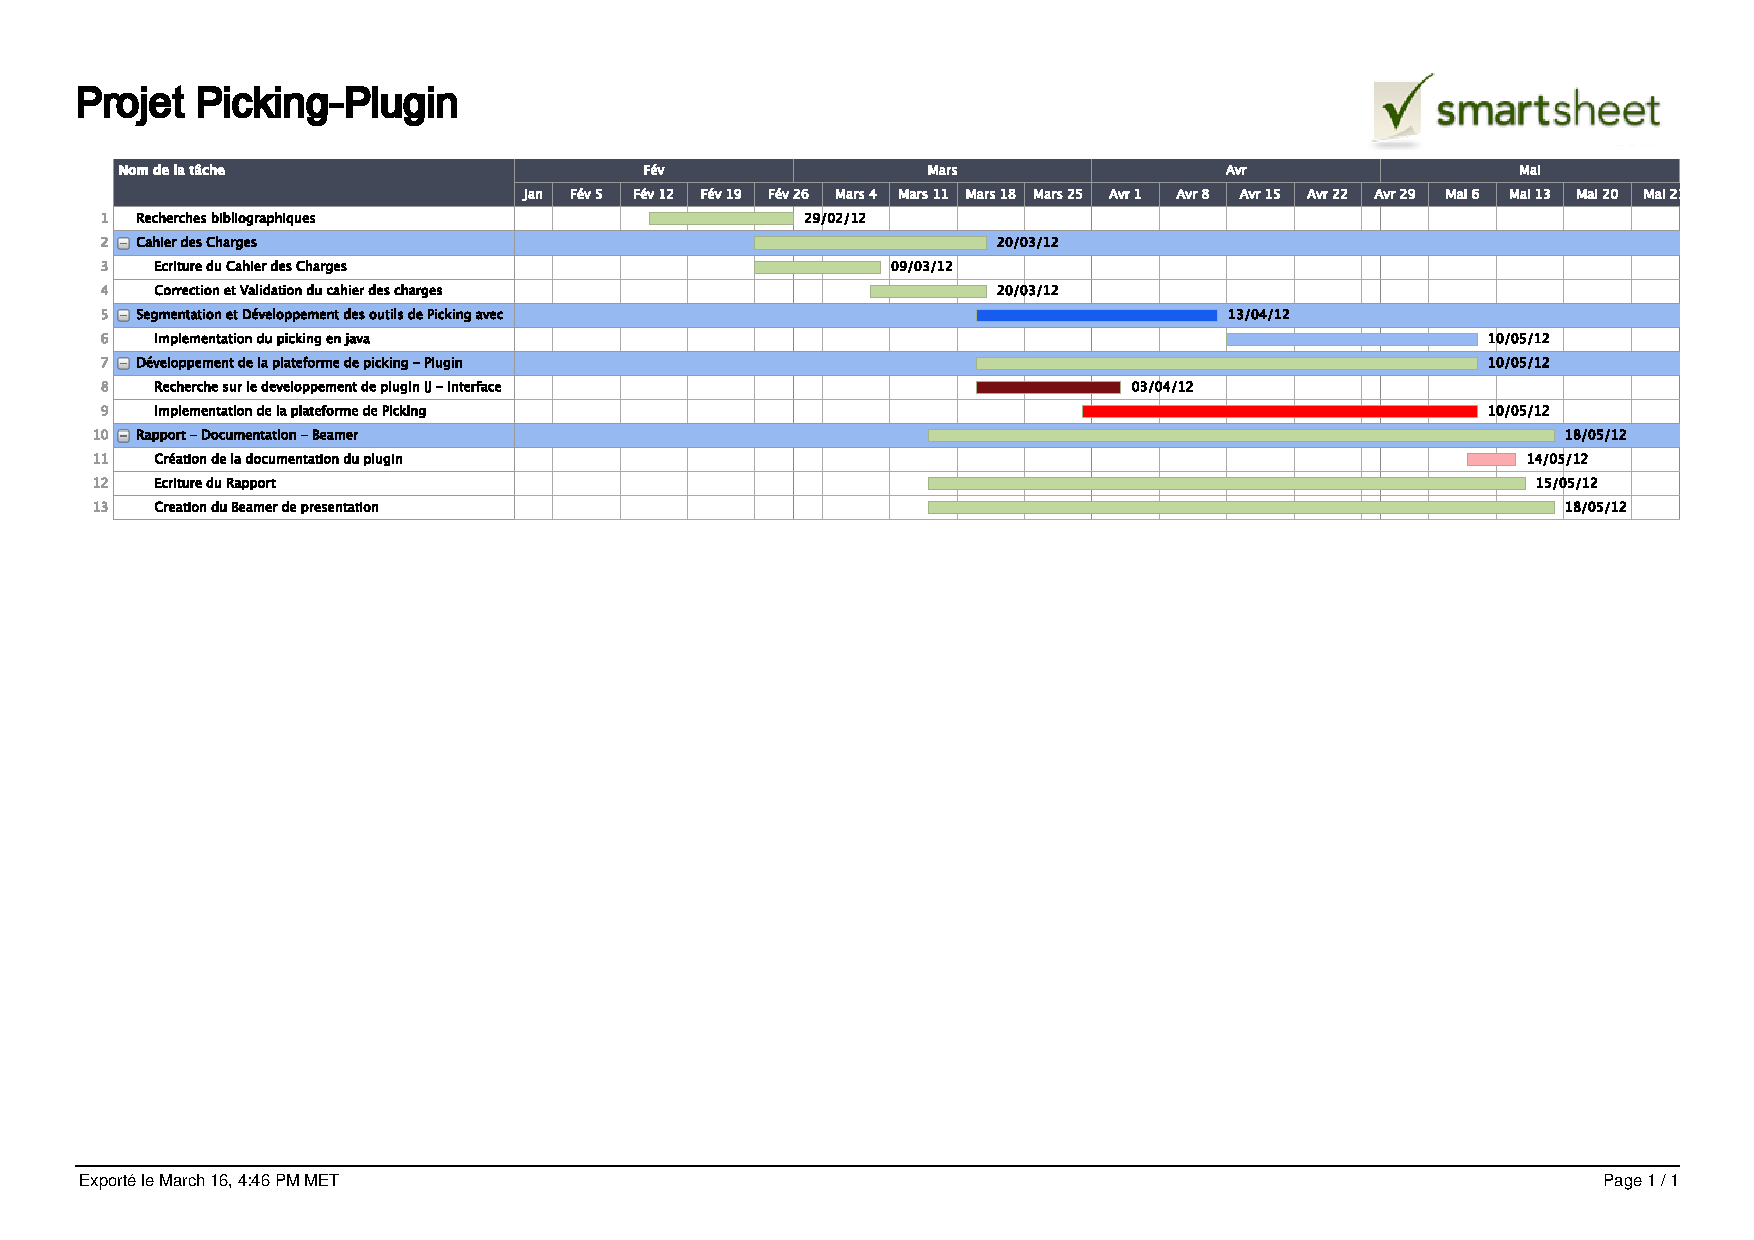
\includepdf[landscape]{GANTT.pdf}
%\end{rotate}
\end{document}